% Template originaly created by Karol Kozioł (mail@karol-koziol.net) and modified for ShareLaTeX use
\documentclass[a4paper,landscape]{article}
\usepackage[T1]{fontenc}
\usepackage[utf8]{inputenc}
\usepackage{graphicx}
\usepackage{sectsty}
\usepackage{tgtermes}
\usepackage{tikz}
\usepackage{xcolor}
\usepackage{lipsum} % for loop
\usepackage{multicol}
\usepackage{fancyvrb}
\usepackage{geometry}
\usepackage{enumerate}
\usepackage{subcaption}
\usepackage[percent]{overpic}
\usepackage{amsmath,amssymb,amsthm,textcomp}
\usepackage[font=large,labelfont={bf,it},textfont=it]{caption}

\usepackage[ pdftitle={Leptonic MonoTop}, pdfauthor={fdolek}, colorlinks=true,linkcolor=blue,urlcolor=blue,citecolor=blue,bookmarks=true, bookmarksopenlevel=2]{hyperref}

% redefine \VerbatimInput
\RecustomVerbatimCommand{\VerbatimInput}{VerbatimInput}%
{fontsize=\footnotesize,
 %
 frame=lines,  % top and bottom rule only
 framesep=2em, % separation between frame and text
  rulecolor=\color{black},
 %
% label=\fbox{\color{black}data.txt},
 labelposition=topline,
 %
 commandchars=\|\(\), % escape character and argument delimiters for
                      % commands within the verbatim
 commentchar=*        % comment character
}



\geometry{total={210mm,297mm},
left=5mm,right=5mm,%
bindingoffset=0mm, top=5mm,bottom=5mm}


\linespread{1.3}

\newcommand{\linia}{\rule{\linewidth}{0.7pt}}

% custom theorems if needed
\newtheoremstyle{mytheor}
    {1ex}{1ex}{\normalfont}{0pt}{\scshape}{.}{1ex}
    {{\thmname{#1 }}{\thmnumber{#2}}{\thmnote{ (#3)}}}

\theoremstyle{mytheor}
\newtheorem{defi}{Definition}

% my own titles
\makeatletter
\renewcommand{\maketitle}{
\begin{center}
\vspace{2ex}
{\huge \textsc{\@title}}
\vspace{1ex}
\\
\linia\\
\@author \hfill \@date
\vspace{4ex}
\end{center}
}
\makeatother
%%%

% custom footers and headers
\usepackage{fancyhdr,lastpage}
\pagestyle{fancy}
\lhead{}
\chead{}
\rhead{}
\lfoot{}
\cfoot{}
\rfoot{Page \thepage\ / \pageref{LastPage}}
\renewcommand{\headrulewidth}{0pt}
\renewcommand{\footrulewidth}{0pt}
%

%%%----------%%%----------%%%----------%%%----------%%%

\begin{document}

%   QAZTITLE and QAZDATE will be replaced by root2pdf program.
\title{decaf 2018} 

\author{lpcDM Team}

\date{\today}

\maketitle

\begin{center}
\textbf{} 


maker 2018 without 


%%%%%%%%%%%%%%%%%%%%%%%%%%%%%%%%%%%%%%%%%%%%%%%%%%%%%%%%%%%%%%%%%%%%%%%%%%%%%%%%%%%%%%%%%
%\clearpage
\begin{figure*}[ht!]
   
    \begin{subfigure}[b]{0.24\textwidth}
        \centering
        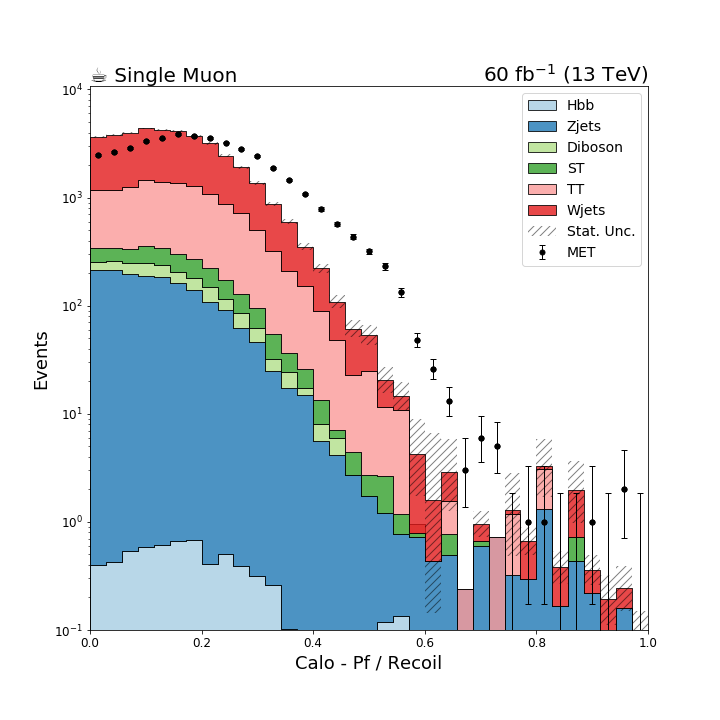
\includegraphics[width=\textwidth]{stack/stackCaloMinusPfOverRecoil.png}
        \caption{test}
    \end{subfigure}
    \quad
    \begin{subfigure}[b]{0.24\textwidth}  
        \centering 
        \includegraphics[width=\textwidth]{2.stackCaloMinusPfOverRecoil.png}
        \caption{}
    \end{subfigure}
    \quad
    \begin{subfigure}[b]{0.24\textwidth}  
        \centering 
        \includegraphics[width=\textwidth]{3.stackCaloMinusPfOverRecoil.png}
        \caption{}
    \end{subfigure}
    \quad
    \begin{subfigure}[b]{0.24\textwidth}  
        \centering 
        \includegraphics[width=\textwidth]{4.stackCaloMinusPfOverRecoil.png}
        \caption{}
    \end{subfigure}
     \caption{CaloMinusPfOverRecoilM}
%%%%%%%%%%%%%%%%%%%%%%%%%%%%%%%%%%%%%%%
    \vskip\baselineskip
    \begin{subfigure}[b]{0.24\textwidth}   
        \centering 
        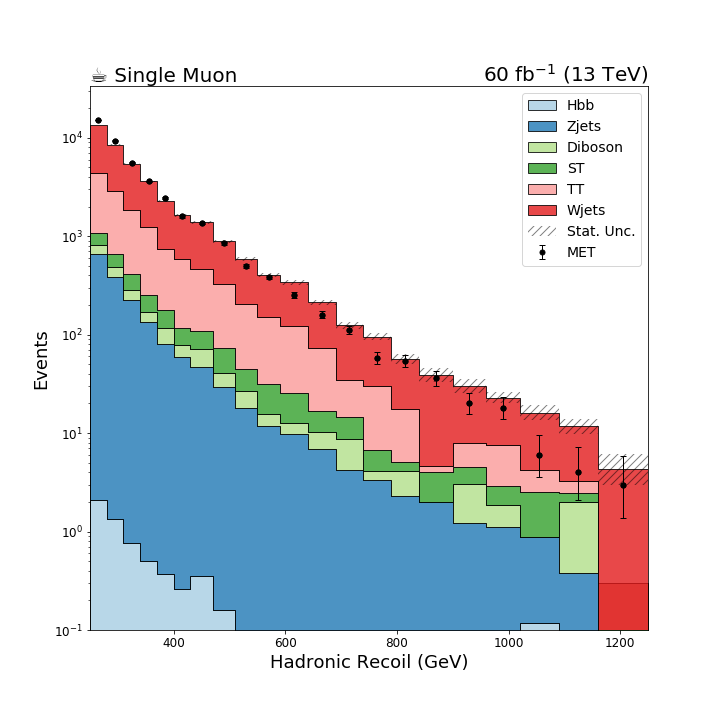
\includegraphics[width=\textwidth]{stack/stackrecoil.png}
        \caption{}
    \end{subfigure}
    \quad
    \begin{subfigure}[b]{0.24\textwidth}   
        \centering 
        \includegraphics[width=\textwidth]{2.stackrecoil.png}
        \caption{}
    \end{subfigure}
    \quad
    \begin{subfigure}[b]{0.24\textwidth}   
        \centering 
        \includegraphics[width=\textwidth]{3.stackrecoil.png}
        \caption{}
    \end{subfigure}
    \quad
    \begin{subfigure}[b]{0.24\textwidth}   
        \centering 
        \includegraphics[width=\textwidth]{4.stackrecoil.png}
        \caption{}
    \end{subfigure}
    \caption{recoil}
\end{figure*}

\clearpage
%%%%%%%%%%%%%%%%%%%%%%%%%%%%%%%%%%%%%%%%%%%%%%%%%%%%%%%%%%%%%%%%%%%%%%%%%%%%%%%%%%%%%%%%%
%\clearpage
\begin{figure*}[ht!]
   
    \begin{subfigure}[b]{0.24\textwidth}
        \centering
        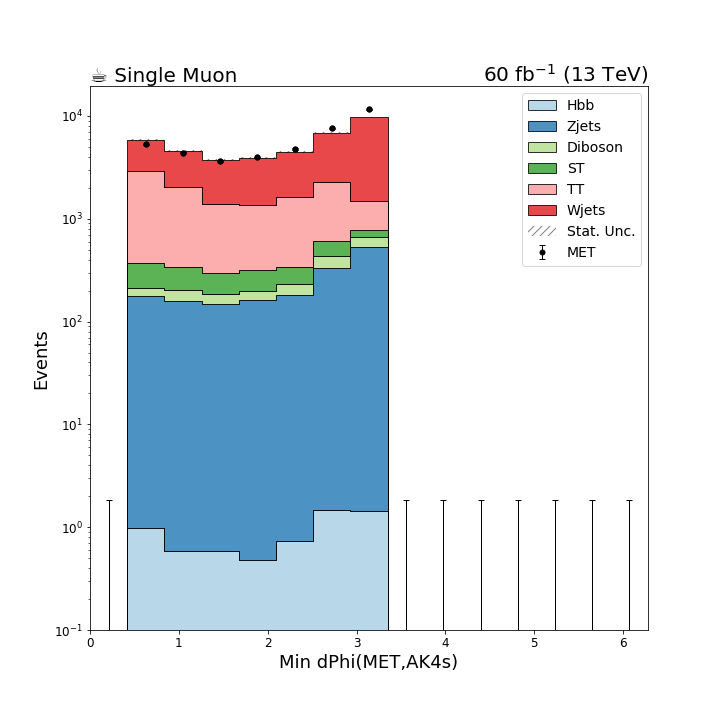
\includegraphics[width=\textwidth]{stack/stackmindphi.png}
        \caption{test}
    \end{subfigure}
    \quad
    \begin{subfigure}[b]{0.24\textwidth}  
        \centering 
        \includegraphics[width=\textwidth]{2.stackmindphi.png}
        \caption{}
    \end{subfigure}
    \quad
    \begin{subfigure}[b]{0.24\textwidth}  
        \centering 
        \includegraphics[width=\textwidth]{3.stackmindphi.png}
        \caption{}
    \end{subfigure}
    \quad
    \begin{subfigure}[b]{0.24\textwidth}  
        \centering 
        \includegraphics[width=\textwidth]{4.stackmindphi.png}
        \caption{}
    \end{subfigure}
     \caption{mindphiM}
%%%%%%%%%%%%%%%%%%%%%%%%%%%%%%%%%%%%%%%
    \vskip\baselineskip
    \begin{subfigure}[b]{0.24\textwidth}   
        \centering 
        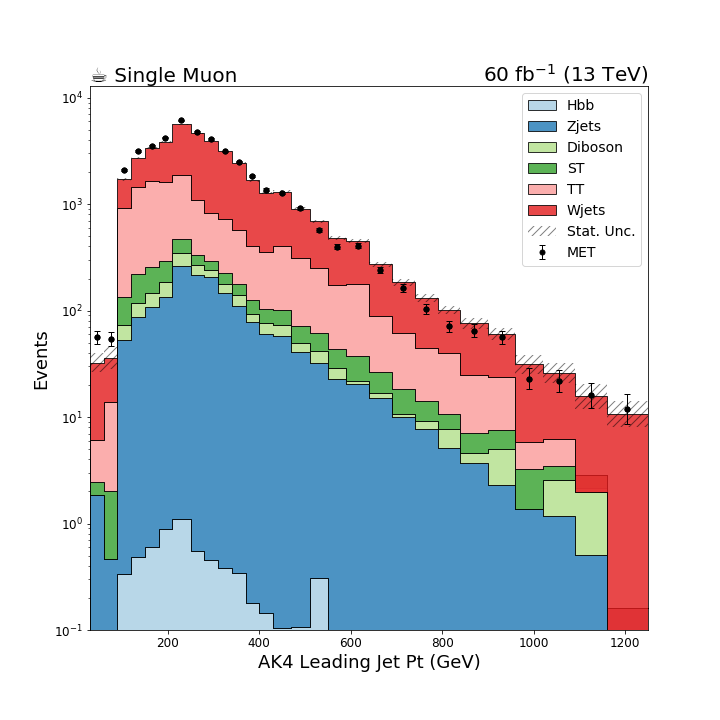
\includegraphics[width=\textwidth]{stack/stackj1pt.png}
        \caption{}
    \end{subfigure}
    \quad
    \begin{subfigure}[b]{0.24\textwidth}   
        \centering 
        \includegraphics[width=\textwidth]{2.stackj1pt.png}
        \caption{}
    \end{subfigure}
    \quad
    \begin{subfigure}[b]{0.24\textwidth}   
        \centering 
        \includegraphics[width=\textwidth]{3.stackj1pt.png}
        \caption{}
    \end{subfigure}
    \quad
    \begin{subfigure}[b]{0.24\textwidth}   
        \centering 
        \includegraphics[width=\textwidth]{4.stackj1pt.png}
        \caption{}
    \end{subfigure}
    \caption{j1pt}
\end{figure*}

\clearpage

%%%%%%%%%%%%%%%%%%%%%%%%%%%%%%%%%%%%%%%%%%%%%%%%%%%%%%%%%%%%%%%%%%%%%%%%%%%%%%%%%%%%%%%%%
%\clearpage
\begin{figure*}[ht!]
   
    \begin{subfigure}[b]{0.24\textwidth}
        \centering
        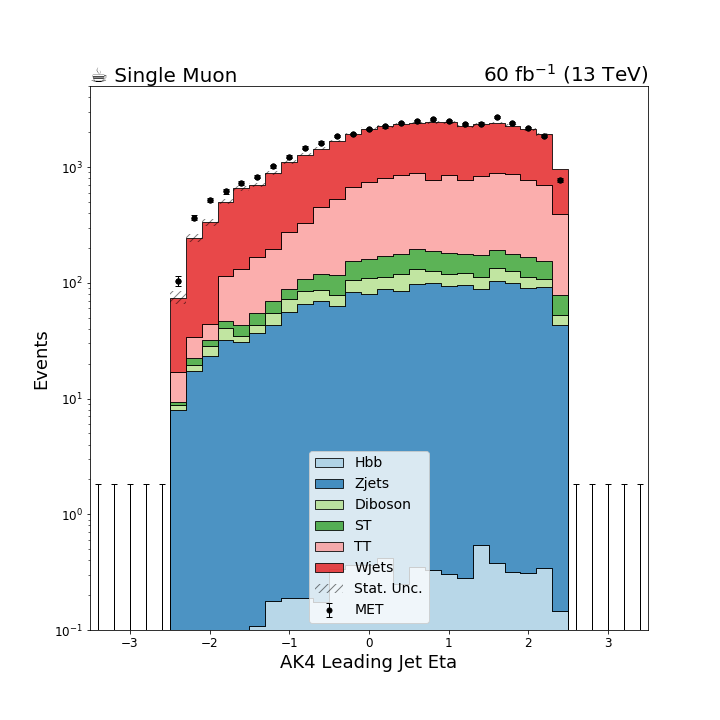
\includegraphics[width=\textwidth]{stack/stackj1eta.png}
        \caption{test}
    \end{subfigure}
    \quad
    \begin{subfigure}[b]{0.24\textwidth}  
        \centering 
        \includegraphics[width=\textwidth]{2.stackj1eta.png}
        \caption{}
    \end{subfigure}
    \quad
    \begin{subfigure}[b]{0.24\textwidth}  
        \centering 
        \includegraphics[width=\textwidth]{3.stackj1eta.png}
        \caption{}
    \end{subfigure}
    \quad
    \begin{subfigure}[b]{0.24\textwidth}  
        \centering 
        \includegraphics[width=\textwidth]{4.stackj1eta.png}
        \caption{}
    \end{subfigure}
     \caption{j1etaM}
%%%%%%%%%%%%%%%%%%%%%%%%%%%%%%%%%%%%%%%
    \vskip\baselineskip
    \begin{subfigure}[b]{0.24\textwidth}   
        \centering 
        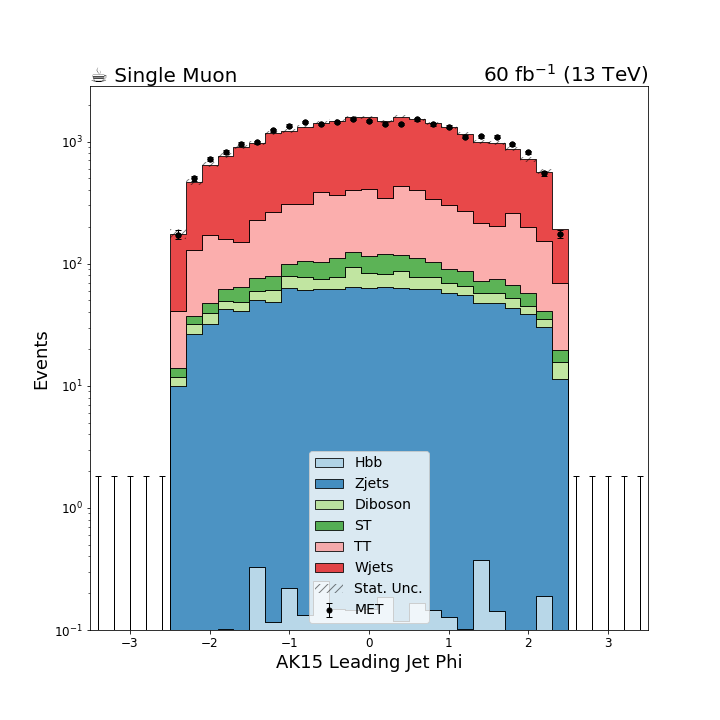
\includegraphics[width=\textwidth]{stack/stackfj1phi.png}
        \caption{}
    \end{subfigure}
    \quad
    \begin{subfigure}[b]{0.24\textwidth}   
        \centering 
        \includegraphics[width=\textwidth]{2.stackfj1phi.png}
        \caption{}
    \end{subfigure}
    \quad
    \begin{subfigure}[b]{0.24\textwidth}   
        \centering 
        \includegraphics[width=\textwidth]{3.stackfj1phi.png}
        \caption{}
    \end{subfigure}
    \quad
    \begin{subfigure}[b]{0.24\textwidth}   
        \centering 
        \includegraphics[width=\textwidth]{4.stackfj1phi.png}
        \caption{}
    \end{subfigure}
    \caption{fj1phi}
\end{figure*}

\clearpage
%%%%%%%%%%%%%%%%%%%%%%%%%%%%%%%%%%%%%%%%%%%%%%%%%%%%%%%%%%%%%%%%%%%%%%%%%%%%%%%%%%%%%%%%%
%\clearpage
\begin{figure*}[ht!]
   
    \begin{subfigure}[b]{0.24\textwidth}
        \centering
        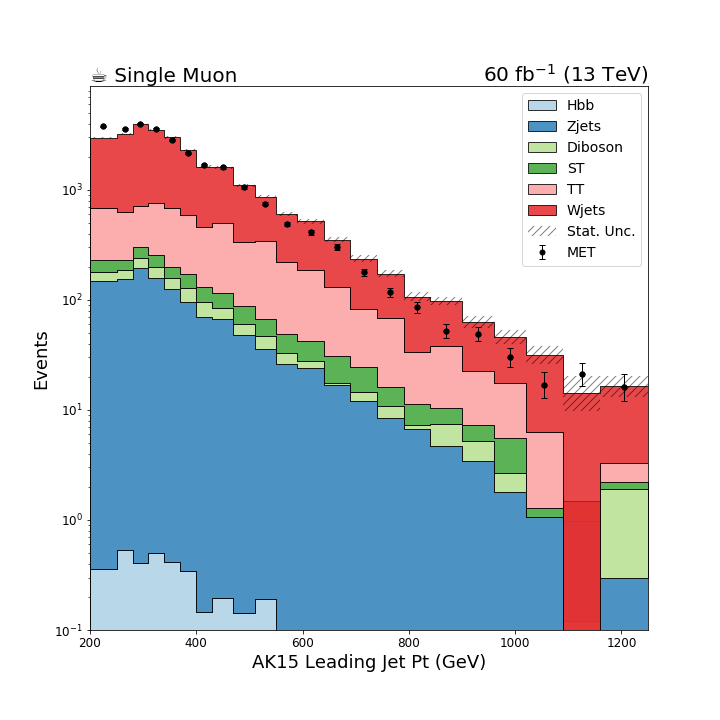
\includegraphics[width=\textwidth]{stack/stackfj1pt.png}
        \caption{test}
    \end{subfigure}
    \quad
    \begin{subfigure}[b]{0.24\textwidth}  
        \centering 
        \includegraphics[width=\textwidth]{2.stackfj1pt.png}
        \caption{}
    \end{subfigure}
    \quad
    \begin{subfigure}[b]{0.24\textwidth}  
        \centering 
        \includegraphics[width=\textwidth]{3.stackfj1pt.png}
        \caption{}
    \end{subfigure}
    \quad
    \begin{subfigure}[b]{0.24\textwidth}  
        \centering 
        \includegraphics[width=\textwidth]{4.stackfj1pt.png}
        \caption{}
    \end{subfigure}
     \caption{fj1ptM}
%%%%%%%%%%%%%%%%%%%%%%%%%%%%%%%%%%%%%%%
    \vskip\baselineskip
    \begin{subfigure}[b]{0.24\textwidth}   
        \centering 
        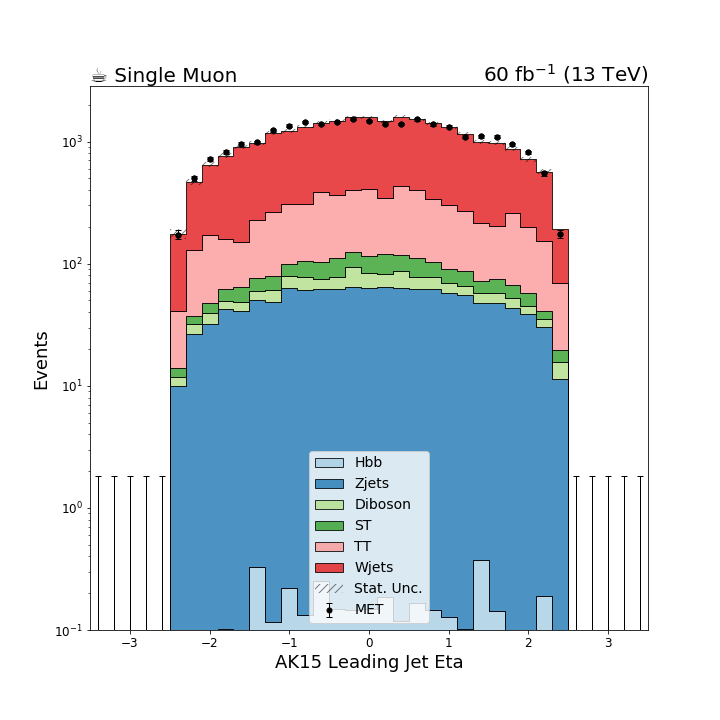
\includegraphics[width=\textwidth]{stack/stackfj1eta.png}
        \caption{}
    \end{subfigure}
    \quad
    \begin{subfigure}[b]{0.24\textwidth}   
        \centering 
        \includegraphics[width=\textwidth]{2.stackfj1eta.png}
        \caption{}
    \end{subfigure}
    \quad
    \begin{subfigure}[b]{0.24\textwidth}   
        \centering 
        \includegraphics[width=\textwidth]{3.stackfj1eta.png}
        \caption{}
    \end{subfigure}
    \quad
    \begin{subfigure}[b]{0.24\textwidth}   
        \centering 
        \includegraphics[width=\textwidth]{4.stackfj1eta.png}
        \caption{}
    \end{subfigure}
    \caption{fj1eta}
\end{figure*}

\clearpage
%%%%%%%%%%%%%%%%%%%%%%%%%%%%%%%%%%%%%%%%%%%%%%%%%%%%%%%%%%%%%%%%%%%%%%%%%%%%%%%%%%%%%%%%%
%\clearpage
\begin{figure*}[ht!]
   
    \begin{subfigure}[b]{0.24\textwidth}
        \centering
        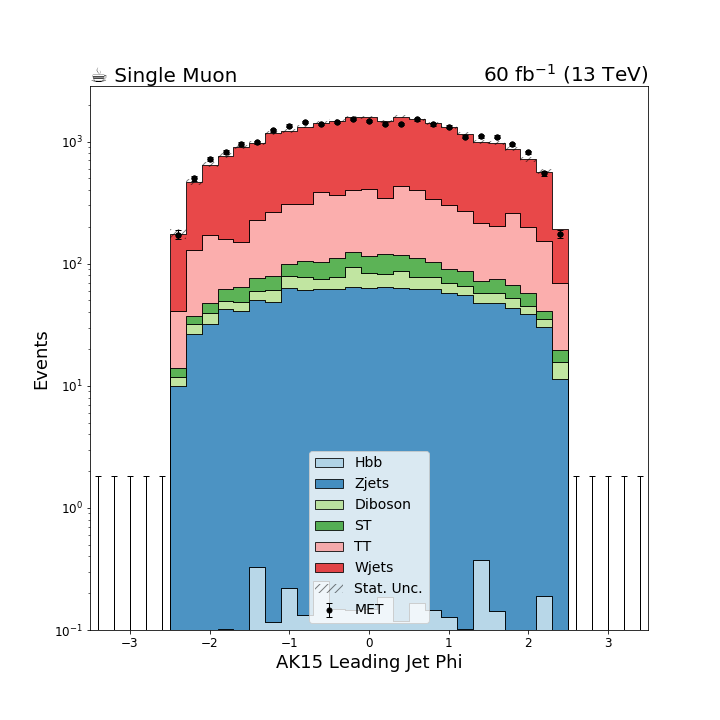
\includegraphics[width=\textwidth]{stack/stackfj1phi.png}
        \caption{test}
    \end{subfigure}
    \quad
    \begin{subfigure}[b]{0.24\textwidth}  
        \centering 
        \includegraphics[width=\textwidth]{2.stackfj1phi.png}
        \caption{}
    \end{subfigure}
    \quad
    \begin{subfigure}[b]{0.24\textwidth}  
        \centering 
        \includegraphics[width=\textwidth]{3.stackfj1phi.png}
        \caption{}
    \end{subfigure}
    \quad
    \begin{subfigure}[b]{0.24\textwidth}  
        \centering 
        \includegraphics[width=\textwidth]{4.stackfj1phi.png}
        \caption{}
    \end{subfigure}
     \caption{fj1phiM}
%%%%%%%%%%%%%%%%%%%%%%%%%%%%%%%%%%%%%%%
    \vskip\baselineskip
    \begin{subfigure}[b]{0.24\textwidth}   
        \centering 
        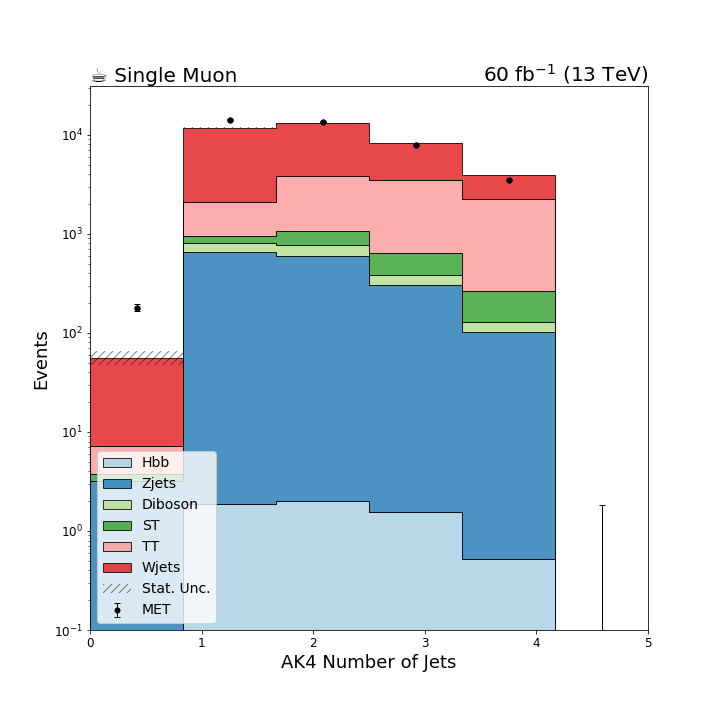
\includegraphics[width=\textwidth]{stack/stacknjets.png}
        \caption{}
    \end{subfigure}
    \quad
    \begin{subfigure}[b]{0.24\textwidth}   
        \centering 
        \includegraphics[width=\textwidth]{2.stacknjets.png}
        \caption{}
    \end{subfigure}
    \quad
    \begin{subfigure}[b]{0.24\textwidth}   
        \centering 
        \includegraphics[width=\textwidth]{3.stacknjets.png}
        \caption{}
    \end{subfigure}
    \quad
    \begin{subfigure}[b]{0.24\textwidth}   
        \centering 
        \includegraphics[width=\textwidth]{4.stacknjets.png}
        \caption{}
    \end{subfigure}
    \caption{njets}
\end{figure*}

\clearpage
%%%%%%%%%%%%%%%%%%%%%%%%%%%%%%%%%%%%%%%%%%%%%%%%%%%%%%%%%%%%%%%%%%%%%%%%%%%%%%%%%%%%%%%%%
%\clearpage
\begin{figure*}[ht!]
   
    \begin{subfigure}[b]{0.24\textwidth}
        \centering
        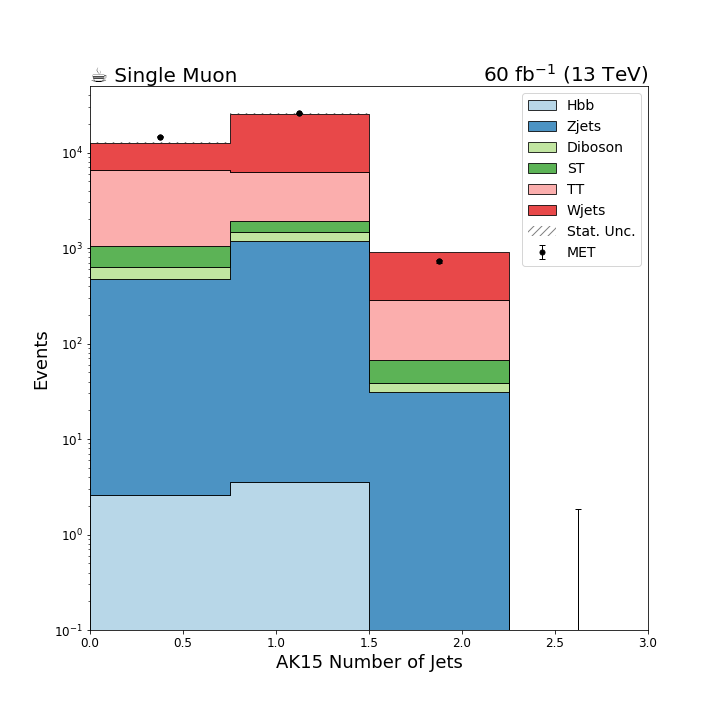
\includegraphics[width=\textwidth]{stack/stacknfjets.png}
        \caption{test}
    \end{subfigure}
    \quad
    \begin{subfigure}[b]{0.24\textwidth}  
        \centering 
        \includegraphics[width=\textwidth]{2.stacknfjets.png}
        \caption{}
    \end{subfigure}
    \quad
    \begin{subfigure}[b]{0.24\textwidth}  
        \centering 
        \includegraphics[width=\textwidth]{3.stacknfjets.png}
        \caption{}
    \end{subfigure}
    \quad
    \begin{subfigure}[b]{0.24\textwidth}  
        \centering 
        \includegraphics[width=\textwidth]{4.stacknfjets.png}
        \caption{}
    \end{subfigure}
     \caption{nfjetsM}
%%%%%%%%%%%%%%%%%%%%%%%%%%%%%%%%%%%%%%%
    \vskip\baselineskip
    \begin{subfigure}[b]{0.24\textwidth}   
        \centering 
        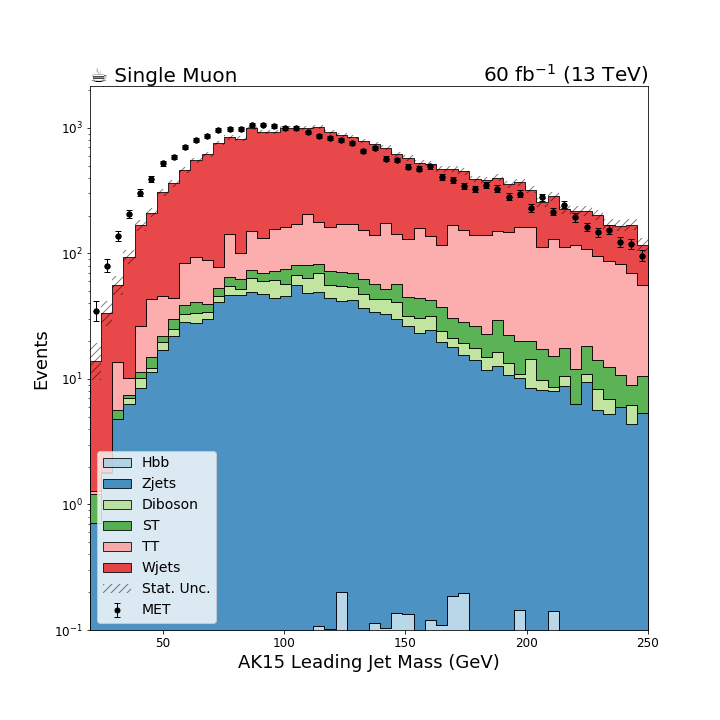
\includegraphics[width=\textwidth]{stack/stackfjmass.png}
        \caption{}
    \end{subfigure}
    \quad
    \begin{subfigure}[b]{0.24\textwidth}   
        \centering 
        \includegraphics[width=\textwidth]{2.stackfjmass.png}
        \caption{}
    \end{subfigure}
    \quad
    \begin{subfigure}[b]{0.24\textwidth}   
        \centering 
        \includegraphics[width=\textwidth]{3.stackfjmass.png}
        \caption{}
    \end{subfigure}
    \quad
    \begin{subfigure}[b]{0.24\textwidth}   
        \centering 
        \includegraphics[width=\textwidth]{4.stackfjmass.png}
        \caption{}
    \end{subfigure}
    \caption{fjmass}
\end{figure*}

\clearpage
%%%%%%%%%%%%%%%%%%%%%%%%%%%%%%%%%%%%%%%%%%%%%%%%%%%%%%%%%%%%%%%%%%%%%%%%%%%%%%%%%%%%%%%%%
%\clearpage
\begin{figure*}[ht!]
   
    \begin{subfigure}[b]{0.24\textwidth}
        \centering
        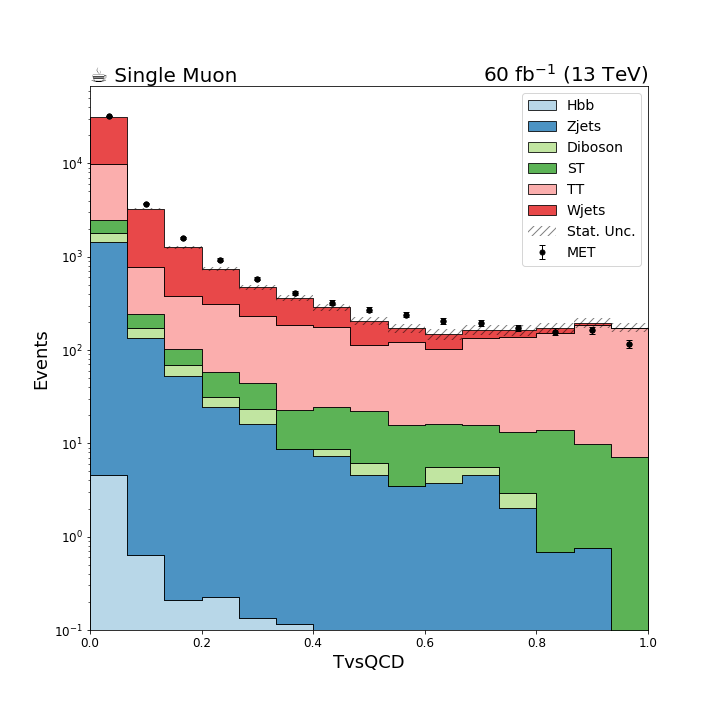
\includegraphics[width=\textwidth]{stack/stackTvsQCD.png}
        \caption{test}
    \end{subfigure}
    \quad
    \begin{subfigure}[b]{0.24\textwidth}  
        \centering 
        \includegraphics[width=\textwidth]{2.stackTvsQCD.png}
        \caption{}
    \end{subfigure}
    \quad
    \begin{subfigure}[b]{0.24\textwidth}  
        \centering 
        \includegraphics[width=\textwidth]{3.stackTvsQCD.png}
        \caption{}
    \end{subfigure}
    \quad
    \begin{subfigure}[b]{0.24\textwidth}  
        \centering 
        \includegraphics[width=\textwidth]{4.stackTvsQCD.png}
        \caption{}
    \end{subfigure}
     \caption{TvsQCDM}
%%%%%%%%%%%%%%%%%%%%%%%%%%%%%%%%%%%%%%%
    \vskip\baselineskip
    \begin{subfigure}[b]{0.24\textwidth}   
        \centering 
        \includegraphics[width=\textwidth]{stack/stackhSvsQCD.png}
        \caption{}
    \end{subfigure}
    \quad
    \begin{subfigure}[b]{0.24\textwidth}   
        \centering 
        \includegraphics[width=\textwidth]{2.stackhSvsQCD.png}
        \caption{}
    \end{subfigure}
    \quad
    \begin{subfigure}[b]{0.24\textwidth}   
        \centering 
        \includegraphics[width=\textwidth]{3.stackhSvsQCD.png}
        \caption{}
    \end{subfigure}
    \quad
    \begin{subfigure}[b]{0.24\textwidth}   
        \centering 
        \includegraphics[width=\textwidth]{4.stackhSvsQCD.png}
        \caption{}
    \end{subfigure}
    \caption{hSvsQCD}
\end{figure*}

\clearpage
%%%%%%%%%%%%%%%%%%%%%%%%%%%%%%%%%%%%%%%%%%%%%%%%%%%%%%%%%%%%%%%%%%%%%%%%%%%%%%%%%%%%%%%%%
%\clearpage
\begin{figure*}[ht!]
   
    \begin{subfigure}[b]{0.24\textwidth}
        \centering
        \includegraphics[width=\textwidth]{stack/stackVvsQCD.png}
        \caption{test}
    \end{subfigure}
    \quad
    \begin{subfigure}[b]{0.24\textwidth}  
        \centering 
        \includegraphics[width=\textwidth]{2.stackVvsQCD.png}
        \caption{}
    \end{subfigure}
    \quad
    \begin{subfigure}[b]{0.24\textwidth}  
        \centering 
        \includegraphics[width=\textwidth]{3.stackVvsQCD.png}
        \caption{}
    \end{subfigure}
    \quad
    \begin{subfigure}[b]{0.24\textwidth}  
        \centering 
        \includegraphics[width=\textwidth]{4.stackVvsQCD.png}
        \caption{}
    \end{subfigure}
     \caption{VvsQCDM}
%%%%%%%%%%%%%%%%%%%%%%%%%%%%%%%%%%%%%%%
    \vskip\baselineskip
    \begin{subfigure}[b]{0.24\textwidth}   
        \centering 
        \includegraphics[width=\textwidth]{1.png}
        \caption{}
    \end{subfigure}
    \quad
    \begin{subfigure}[b]{0.24\textwidth}   
        \centering 
        \includegraphics[width=\textwidth]{2.png}
        \caption{}
    \end{subfigure}
    \quad
    \begin{subfigure}[b]{0.24\textwidth}   
        \centering 
        \includegraphics[width=\textwidth]{3.png}
        \caption{}
    \end{subfigure}
    \quad
    \begin{subfigure}[b]{0.24\textwidth}   
        \centering 
        \includegraphics[width=\textwidth]{4.png}
        \caption{}
    \end{subfigure}
    \caption{png}\end{figure*}

\clearpage




QC_DHT100to200_TuneCUETP8M1_13TeV-madgraphMLM-pythia8/
8021 - FileReadError (May be a site error)

QCD_HT700to1000_TuneCUETP8M1_13TeV-madgraphMLM-pythia8-ext1/
8028 - FileOpenError with fallback 



\end{document} 
